% Chapter Template

\chapter{Conclusion} % Main chapter title

\label{Chapter6} % Change X to a consecutive number; for referencing this chapter elsewhere, use \ref{ChapterX}

\lhead{Chapter 6. \emph{Conlusion}} % Change X to a consecutive number; this is for the header on each page - perhaps a shortened title

\rule{\textwidth}{0.4pt} \\[0.5cm]
\textit{``The true face of Lushan is lost to my sight, for it is right in this mountain that I reside."}

\begin{flushright}
Su Shi
\end{flushright}
\rule{\textwidth}{0.4pt} 

In previous chapters, structured domains were dealt with different forms and correspondingly computed with different methods.   
The contributions of this dissertation are twofold. The first one is practical, along with a number of experiments on practical tasks, some basic 
principles in the modeling and computation of structured data are illustrated. The second one, however, is relative theoretic, several        
novel models and learning algorithms were proposed, gaining deeper insights into structured-output learning problems.           

After going through four technical chapters, it is useful to step outside and look at the big picture.    
Although the dissertation is organized with three separate parts: inference, learning and optimization, one can be already 
aware of that they are highly connected.                
Some connections can be listed as follows:  
\begin{itemize}
    \item A Bayesian network can be considered as a special case of a Markov network with conditional distributions as its potential functions;        
	\item conditional random fields are related to max-margin Markov networks;
	\item a max-margin Markov network is essentially equivalent to structural SVM;  
	\item joint SVM is a special case of structural SVM on multi-label learning with linear output kernels;        
	\item learning undirected graphical models with maximum likelihood estimation is highly dependent on the inference performance, for example, 
		persistent Sequential Monte Carlo is a learning algorithm based on sampling-based inference;            
	\item optimization of graphical models using max-product (loopy) belief propagation is an extension of (loopy) belief propagation inference.     
\end{itemize}
All connections are also visualized in Figure \ref{fig:conclusion}. It can be seen that working with structured data itself is a 
structure where different topics can interact each other. For example, better inference can improve learning performance while better learning 
can make inference-based prediction more accurate; a good learning method for max-margin Markov networks can be also promising for the structural SVM and 
vice verse.  
\begin{figure}[h]
	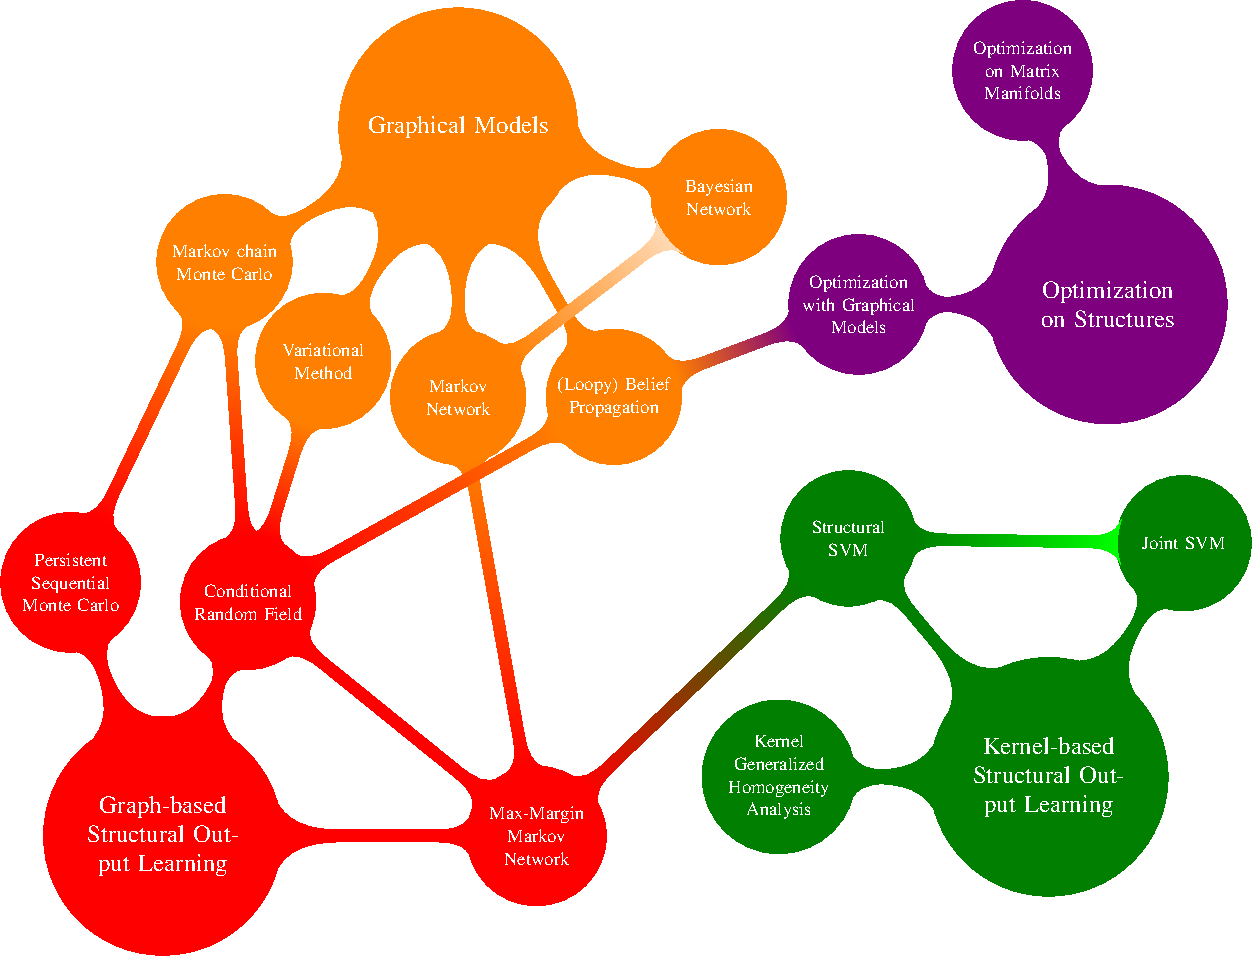
\includegraphics[width=\textwidth]{./Figures/Conclusion_figure-crop}
\caption{How different chapters and sections relate to each other.  }
\label{fig:conclusion}
\end{figure}


Therefore, the main message delivered from the dissertation is to keep a ``structure" mind when confronting multiple data.       
Given a task, based on its nature or characteristic, a structure form is selected and some components in Figure \ref{fig:conclusion} will be involved. 
Furthermore, check how the involved components interact with other ones in the diagram, and then improve the performance by exploiting 
their connections. 

Above all, the content presented in this dissertation is limited. There exist more studies which are influential in relevant       
areas. Also, more developments of working on structured data are expected with increasingly strong desires in practice.        

